\documentclass{article}

\usepackage{graphicx}
\usepackage{tikz}
\usepackage{tikzsymbols}
\usetikzlibrary{calc,patterns,shapes.geometric}
\pagestyle{empty}
\usepackage[margin=0pt]{geometry}
\geometry{papersize={14in,12in}}

\def\centerarc[#1](#2)(#3:#4:#5){\draw[#1] ($(#2)+({#5*cos(#3)},{#5*sin(#3)})$) arc (#3:#4:#5);}

\begin{document}
	\begin{figure}
		\centering
		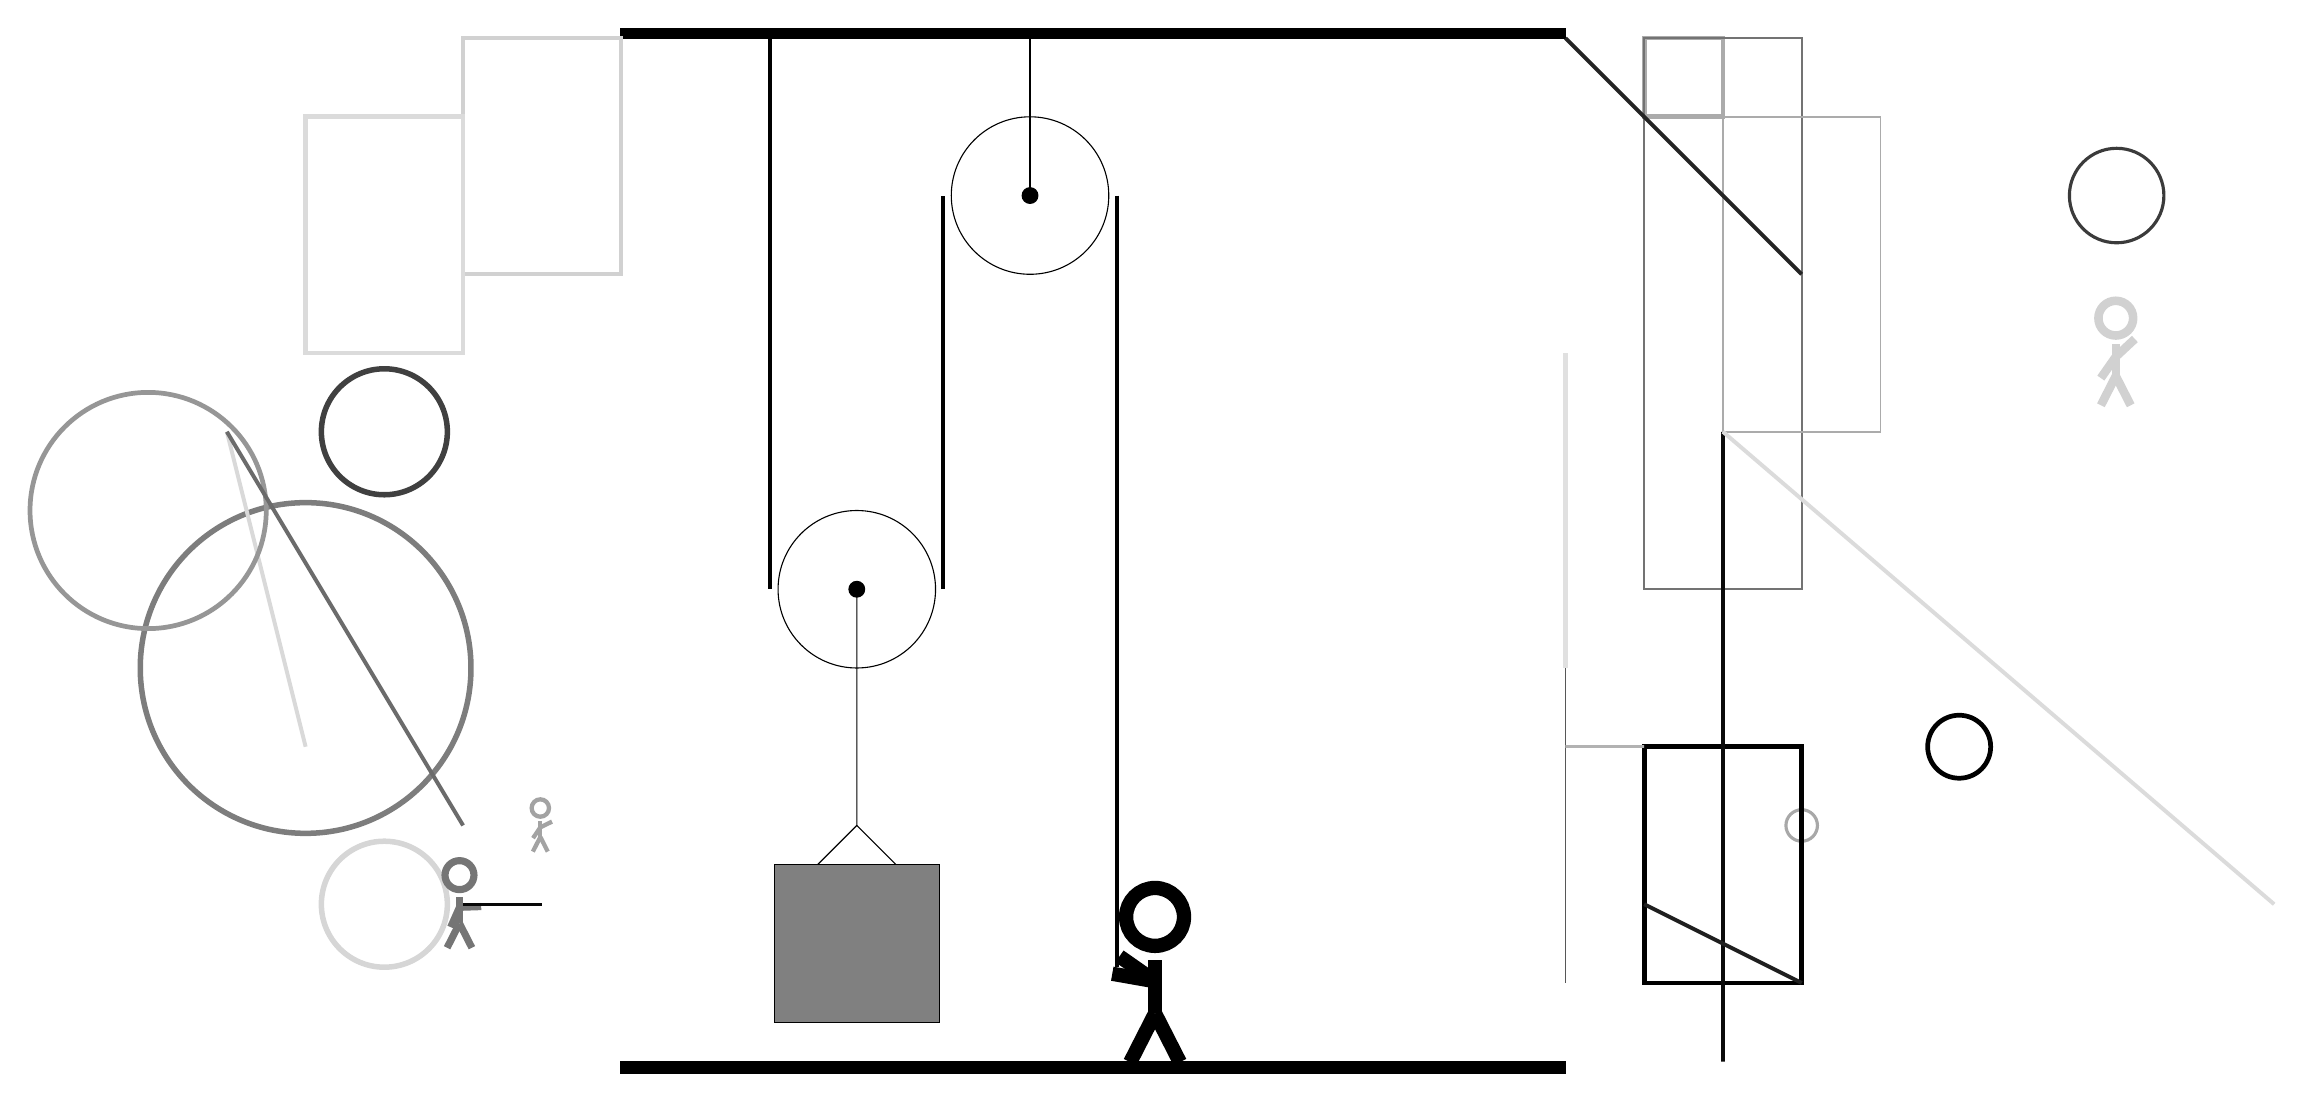
\begin{tikzpicture}
			%%%%% START %%%%%
			
			\draw[fill=black] (-2, 10) rectangle (10, 10.125);
			
			\draw (3.2, 8.0) circle (1);
			\draw[fill=black] (3.2, 8.0) circle (0.1);
			\draw[thick] (3.2, 8.0) -- (3.2, 10);
			
			\draw (1, 3.0) circle (1);
			\draw[fill=black] (1, 3.0) circle (0.1);
			
			\draw (1, 3.0) -- (1, 0) -- (0.5, -0.5);
			\draw (1, 0) -- (1.5, -0.5);
			\draw[fill=black!50] (-0.05, -0.5) rectangle (2.05, -2.5);
			
			\draw [line width=0.7mm, color=black!51](-6, 2) circle (2.1);
			
			\draw [line width=0.6mm, color=black!100](15, 1) circle (0.4);
			\draw [line width=0.4mm, color=black!34](13, 0) circle (0.2);
			\node[line width=0.7mm, color=black!18] at (17, 6) {\Strichmaxerl[6][55][43]};
			
			\draw[line width=0.6mm, color=black!100] (11, 1) rectangle (13, -2);
			\draw[line width=0.5mm, color=black!15](-6, 1) -- (-7, 5);
			\draw[line width=0.6mm, color=black!33] (11, 9) rectangle (12, 10);
			\draw[line width=0.2mm, color=black!66] (10, 6) rectangle (10, -2);
			\draw [line width=0.7mm, color=black!16](-5, -1) circle (0.8);
			\draw [line width=0.6mm, color=black!41](-8, 4) circle (1.5);
			\draw[line width=0.3mm, color=black!55] (11, 10) rectangle (13, 3);
			\draw[line width=0.4mm, color=black!96] (12, -3) rectangle (12, 5);
			\node[line width=0.6mm, color=black!36] at (-3, 0) {\Strichmaxerl[3][56][26]};
			\draw[line width=0.6mm, color=black!12] (10, 6) rectangle (10, 2);
			\draw[line width=0.4mm, color=black!30] (11, 1) rectangle (10, 1);
			\draw[line width=0.2mm, color=black!33] (12, 9) rectangle (14, 5);
			
			\draw[line width=0.5mm, color=black!18] (-4, 10) rectangle (-2, 7);
			\draw[line width=0.5mm, color=black!88](11, -1) -- (13, -2);
			\draw[line width=0.5mm, color=black!86](10, 10) -- (13, 7);
			\draw[line width=0.5mm, color=black!58](-7, 5) -- (-4, 0);
			\draw [line width=0.7mm, color=black!75](-5, 5) circle (0.8);
			
			\draw[line width=0.5mm, color=black!14](12, 5) -- (19, -1);
			
			\node[line width=0.2mm, color=black!54] at (-4, -1) {\Strichmaxerl[5][66][2]};
			\draw[line width=0.6mm, color=black!14] (-4, 6) rectangle (-6, 9);
			\draw [line width=0.4mm, color=black!77](17, 8) circle (0.6);
			
			\draw[line width=0.4mm, color=black!97] (-3, -1) rectangle (-4, -1);
			
			\draw[line width=0.5mm] (-0.1, 10) -- (-0.1, 3.0);
			\centerarc[line width=0.5mm](1, 3.0)(180:360:1.1);
			\draw[line width=0.5mm](2.1, 3.0) -- (2.1, 8.0);
			\centerarc[line width=0.5mm](3.2, 8.0)(0:180:1.1);
			\draw[line width=0.5mm](4.3, 8.0) -- (4.3, -1.8);
			
			\node at (4.7, -1.9) {\Strichmaxerl[10][-35][170]};
			
			\draw[fill=black] (-2, -3) rectangle (10, -3.15);
			
			%%%%% END %%%%%
		\end{tikzpicture}
	\end{figure}	
\end{document}